%!TEX root=paper/paper.tex
\chapter{Conclusion}\label{sec:conclusion}

\PM{Main Contribution}
We note a significant problem that has received little research attention: Anytime visual recognition.
The problem is motivated by the properties of human visual perception and by the need to effectively schedule computationally expensive state-of-the-art computer vision methods for different computational budgets.
We approach the problem from the perspective of reinforcement learning, and successfully learn fully general policies for selecting detector and classifier actions.
To evaluate our approaches, we introduce a new metric of Anytime performance, based on the area under the performance vs. cost curve.
In all experiments, we show that having a dynamic state (and thus allowing ``closed-loop'' policies) and planning ahead increases performance.

\PM{Detection}
We present a method for learning closed-loop policies for multi-class object detection, given existing object detectors and classifiers and a metric to optimize.
The method learns the optimal policy using reinforcement learning, by observing execution traces in training.
As with most reinforcement learning problems, the reward function is defined manually, with domain knowledge.
Here, we derive it for the novel detection AP vs. Time evaluation that we suggest is useful for evaluating efficiency in recognition.
If detection on an image is cut off after only half the detectors have been run, our method does $66\%$ better than a random ordering, and $14\%$ better than an intelligent baseline.
In particular, our method learns to take action with no intermediate reward in order to improve the overall performance of the system.

\PM{Classification}
For the classification task, we need to use a different inference mechanism and additionally need to train classifiers for partially-observed sets of features.
We investigate methods such as different forms of imputation and classifier clustering for this task, and adjust the reward function and the featurization of the state.
Using our method, we show improved Anytime performance on a synthetic classification task and two benchmark visual recognition tasks.
Furthermore, on a hierarchically-structured dataset, we show that accuracy of predictions can be held constant for all budgets, while the specificty of predictions increases.

\PM{Anytime CNN Detection}
Even the most recent state-of-the-art CNN-based detection methods are computationally expensive.
We first consider approaches which can effectively reorder the sequence of regions to maximize the chance that correct detections will be found early, based on inference from relatively lightweight features.
We show that basic strategies, such as simply reordering the boxes such that they do not have a degenerate spatial layout, provides a surprising boost, and that very simple features such as region and gradient statistics can effectively prioritize regions.
Our main contribution is the Cascade CNN model, which adds a novel Reject layer between convolutional layers in the architecture.
C-CNN obtains an 8x speedup of the R-CNN detection method with only a 10\% degradation of state-of-the-art performance on PASCAL VOC detection.

\PM{Recognizing Style}
We have also made significant progress in defining the problem of recognizing image style.
We provide a novel dataset of several types of visual style -- including for visual art -- not previously considered in the literature.
In preparation for an Anytime approach, we evaluate several types of visual features on the dataset, and demonstrate state-of-the-art results in prediction of both style and aesthetic quality (on an existing dataset).
We confirm that our results are comparable to human performance, show that style is highly content-dependent, and demonstrate an image search application where results are queried by content and filtered by style.

\section{Future Work}

\subsection{Detection and Classification}

\PM{Decision Cost}
Computation devoted to scheduling actions is far less significant than the computation due to running the actions in all of our work, and our framework does not explicitly consider this decision-making cost.
However, a welcome extension would explicitly model the decision cost by drawing on existing theoretical work on meta-reasoning (such as \cite{Hay2012}).
Interesting extensions could try to balance the cost of inference vs. the expected gain in efficiency.

\PM{NN Methods}
Nearest-neighbor methods are well suited to settings with partially observed sets of features, and so could be a good addition to our work on Anytime classification.
However, naive NN methods are too slow for our purposes, and we did not evaluate them.
Locality-sensitive hashing methods such as \cite{Kulis2009b} may be an effective solution.
In particular, the original method of \cite{Gao-NIPS-2011} could potentially be extended with hashing to maintain its model-free advantages over a rigidly parametrized model at an acceptable speed.

\PM{Perception}
Beyond the aspects of practical deployment of vision systems that our work is motivated by, we are curious to further investigate our model as a tool to study human cognition and the time course of visual perception.
Only a few attempts have been made to explain this: for example, via sequential decision processes in \textcite{Hegde-Neuro-2008}.
While we have not made any claims about the biological mechanism of perception, our work in reinforcement learning-based feature selection as well as convolutional neural networks has explanatory potential if more tightly integrated in future work.

\PM{Adaptive Submodularity}
The most intriguing future direction is in theoretical analysis of our Anytime method.
Our MDP-based formulation is empirically successful, but fundamentally heuristic.
Adaptive submodularity \parencite{Golovin-and-Krause-2010-JAIR}, a recently developed framework for obtaining famous near-optimality results of \cite{Nemhauser1978} in the context of learning policies.
Just as that work proved that greedy selection can be near-optimal if some conditions of the set function are satisfied, \cite{Golovin-and-Krause-2010-JAIR} prove that greedy policies can also be near-optimal under certain conditions.
Unfortunately, designing an appropriate objective function for our task of visual recognition is not straightforward.

\PM{Submodular Ideas}
Information gain, a component of our reward function, can be shown to not be submodular \cite{Krause-UAI-2005}, so the easy solution has a roadblock.
The most promising way forward is pointed by recent work on active learning and robotic grasping.
In \cite{Golovin-2010}, an adaptively submodular objective based on hypothesis space pruning is developed for an active learning task.
In \cite{Javdani2012}, robotic grasping is linked to a submodular set cover problem --- and another set cover analogy is developed in \cite{Chen-2014-ICML} for the problem of picking computer vision detections to evaluate with an oracle.
An adaptively submodular objective for the general classification problem seems close.
Alternatively, we could show that our reward function is empirically submodular -- but that is not as interesting.

\subsection{CNN-based recognition}

\PM{Cascade CNN}
The general structure of the Cascade CNN general structure of simply ``thinning'' input batches as they travel through the network is agnostic to the underlying mechanism.
Although in our work we evaluate on the R-CNN method on the PASCAL dataset, the Cascade CNN can be applied to the SPP-net method of \cite{He-ECCV-2014}, or the part-based method of \cite{Zhang-ECCV-2014}.
In fact, the Cascade CNN can be applied to any existing CNN that predicts in a class-imbalanced domain where speed is important --- speech recognition, for example.

\PM{End-to-end}
Although, the Cascade CNN is shown to be a strong method for speeding up CNN-based detection approaches, its layers were trained in a stage following the initial network training, not in an \emph{end-to-end} fashion that is the hallmark of deep learning models.
Furthermore, the thresholds were set in a separate process, using a special validation set.
Future work should train and set thresholds of the Reject layers at the same time as the other layers are trained, not after the fact.

\begin{figure}[h!]
\begin{center}
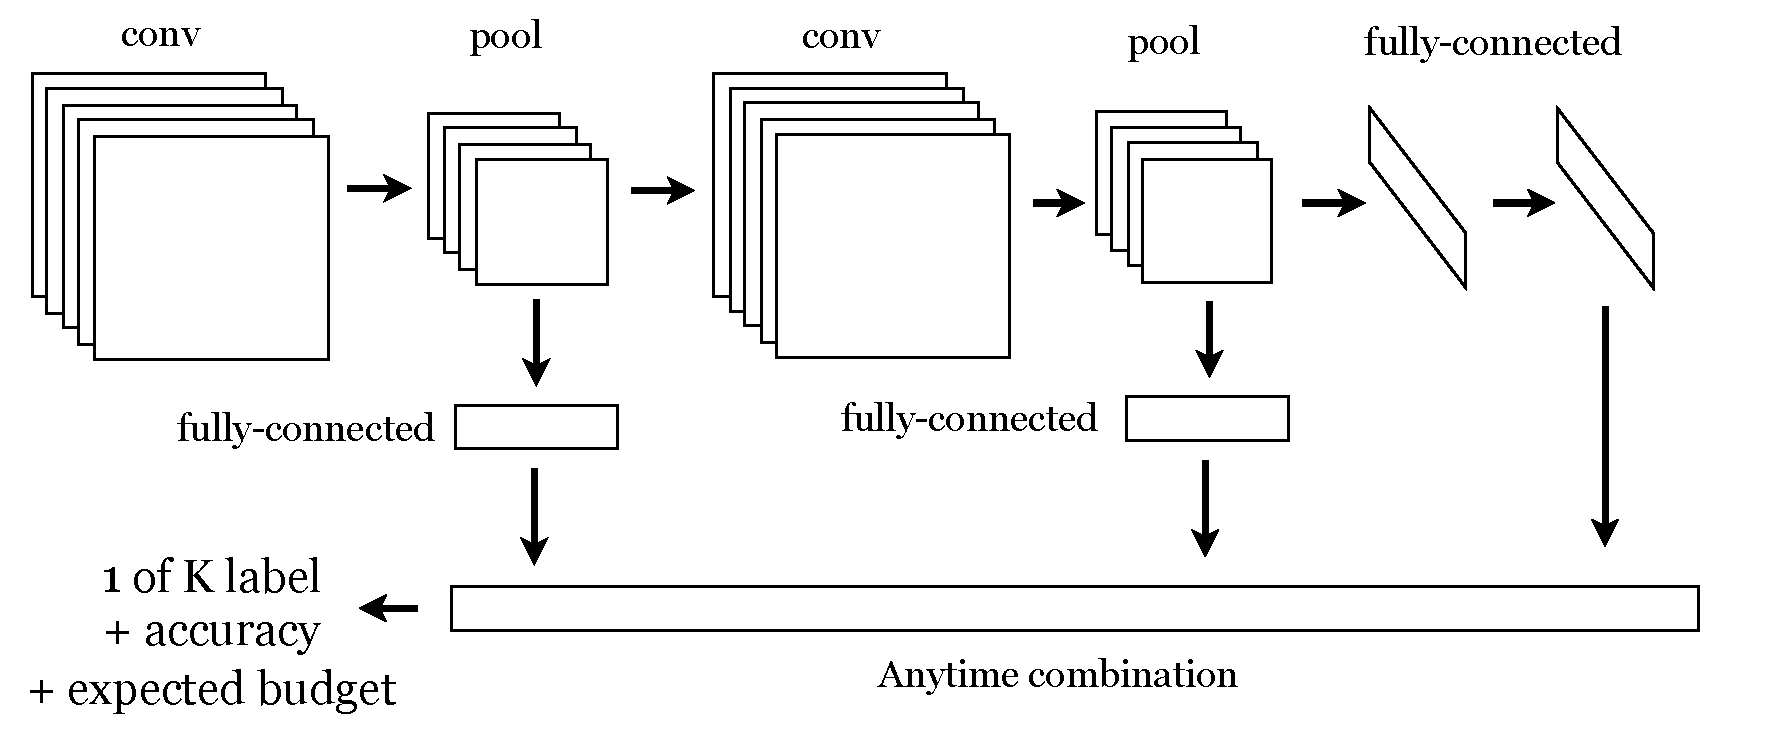
\includegraphics[width=0.98\columnwidth]{../ccnn/figures/ccnn-expanded-anytime.pdf}
\caption[Architecture of the proposed Anytime CNN.]{
The proposed Anytime CNN augments traditional networks with fully-connected prediction layers after every computationally-expensive layer.
All prediction layers feed into an Anytime combination layer that computes accuracy and back-propagates from cost-sensitive loss.
Compare this architecture to \autoref{fig:ccnn}.
}\label{fig:ccnn_anytime}
\end{center}
\end{figure}


\PM{Anytime loss}
More interestingly, networks could be augmented with an ``Anytime loss'' layer that combines classification output from multiple levels of the network in a cost-sensitive way.
This would allow optimizing classification networks for arbitrary distributions of cost budgets.
\autoref{fig:ccnn_anytime} shows the idea: the new layer combines the outputs of all fully-connected layers, which are regularly placed throughout the network.
The Anytime loss computes the expected accuracy of each prediction, takes into account the computational cost up to that layer of the network, and back-propagates according to the budget (for example, if no answers are allowed after 50 ms, and it takes 60 ms to get through the network fully, then the final fully connected layer predictions are never counted).
This setup allows for modeling a distribution over budgets.

\subsection{Image Style}
\PM{Anytime}
While we collected two datasets and showed first results on the challenging new task of recognizing image style, we did not evaluate Anytime performance of our features.
Part of the reason was that one of the most interesting outcomes of this work was the success of features trained on object categorization datasets, and in particular the CNN-based feature.
Although we make a separate Anytime contribution to the CNN in \autoref{sec:ccnn_chapter}, it would still be interesting to evaluate Anytime performance of other visual features on the style datasets.

\PM{Features}
We propose several possible hypotheses to explain the success of general multi-layer features on the style dataset, despite not having been trained on the style task.
Perhaps the network layers that we use as features are extremely good as general visual features for image representation in general.
Another explanation is that object recognition depends on object appearance, e.g., distinguishing red from white wine, or different kinds of terriers, and that the model learns to repurpose these features for image style.
Understanding and improving on these results is fertile ground for future work.
